% This is samplepaper.tex, a sample chapter demonstrating the
% LLNCS macro package for Springer Computer Science proceedings;
% Version 2.21 of 2022/01/12
%
\documentclass[runningheads]{llncs}
%
\usepackage[T1]{fontenc}
% T1 fonts will be used to generate the final print and online PDFs,
% so please use T1 fonts in your manuscript whenever possible.
% Other font encondings may result in incorrect characters.
%
\usepackage{amsmath}
\usepackage{graphicx}
% Used for displaying a sample figure. If possible, figure files should
% be included in EPS format.
%
% If you use the hyperref package, please uncomment the following two lines
% to display URLs in blue roman font according to Springer's eBook style:
%\usepackage{color}
%\renewcommand\UrlFont{\color{blue}\rmfamily}
%\urlstyle{rm}
%
\begin{document}
%
\title{Classificador de Textos com Redes Neurais Profundas}
%
%\titlerunning{Abbreviated paper title}
% If the paper title is too long for the running head, you can set
% an abbreviated paper title here
%
\author{Carlos da Mota Bergueira\inst{1} \and
Diego Jefferson Mendes Silva\inst{1} \and
Filipa Araújo Pereira\inst{1} \and
Rui Manuel Martins Marques Rodrigues\inst{1}}
%
\authorrunning{C. M. Bergueira et al.}
% First names are abbreviated in the running head.
% If there are more than two authors, 'et al.' is used.
%
\institute{Universidade do Minho, Braga, Portugal \\
\email{pg11605@alunos.uminho.pt, pg59999@alunos.uminho.pt, pg42201@alunos.uminho.pt, pg7942@alunos.uminho.pt}}
%
\maketitle              % typeset the header of the contribution
%
\begin{abstract}
Este trabalho aborda o problema de classificação de origem textual em cenário multiclasse, distinguindo textos escritos por humanos de textos gerados automaticamente e, neste último caso, identificando a família do modelo gerador (Anthropic, Google, Meta ou OpenAI). Para esse fim, foi definida uma pipeline supervisionada com recolha e integração de múltiplos datasets públicos, balanceamento de classes e divisão estratificada de treino e avaliação. No pré-processamento, foram exploradas representações vetoriais baseadas em TF-IDF (palavra e caráter), complementadas por \textit{features} estilométricas e estatísticas.

Do ponto de vista metodológico, foram comparadas diferentes famílias de modelos: um \textit{baseline} linear regularizado, uma DNN implementada de raiz em NumPy, uma DNN em PyTorch, um Transformer encoder treinado para a tarefa e um modelo pré-treinado RoBERTa ajustado por \textit{fine-tuning}. A comparação foi conduzida com métricas de classificação multiclasse, com ênfase em \textit{accuracy} e \(F1\)-macro, analisando também estabilidade por classe.

Como principal contribuição, o estudo fornece uma análise comparativa entre arquiteturas de diferentes níveis de complexidade, discutindo o compromisso entre custo computacional, capacidade representacional e robustez na classificação de origem textual.

\keywords{Deep Learning \and Text Classification \and Neural Networks \and Natural Language Processing \and Machine Learning \and Artificial Intelligence}
\end{abstract}
%
%
%
\section{Introdução}

A classificação de textos é uma tarefa fundamental em Processamento de Linguagem Natural (PLN), com aplicações que vão desde a filtragem de spam até a análise de sentimentos e detecção de autoria. Com o advento de modelos de linguagem cada vez mais sofisticados, a distinção entre textos gerados por humanos e por máquinas tornou-se um desafio crescente.

Este trabalho tem como objetivo desenvolver e comparar modelos de aprendizagem supervisionada para classificar textos segundo a sua origem, distinguindo produção humana de produção automática. Para textos de origem automática, o trabalho visa identificar a família do modelo gerador, considerando especificamente as famílias de modelos Anthropic, Google, Meta e OpenAI.

Para avaliar diferentes estratégias de representação textual e arquiteturas de classificação, foram desenvolvidos cinco modelos distintos: um \textit{baseline} linear para comparação, dois modelos DNN (um com implementação NumPy pura e outro com PyTorch para validação), e dois modelos baseados em \textit{Transformers} (um genérico treinado do zero e outro baseado em \textit{fine-tuning} de BERT pré-treinado). Esta abordagem permite análise comparativa entre métodos tradicionais e modernos de PLN.

\begin{itemize}
    \item \textbf{Baseline Linear Regularizado}: Implementação de um modelo linear de referência (Regressão Logística com regularização L2) utilizando apenas NumPy, para estabelecer um \textit{benchmark} de desempenho e comparação com métodos mais complexos.
    
    \item \textbf{\textit{Deep Neural Network} (DNN) com NumPy}: Implementação de uma rede neural profunda multiclasse com múltiplas camadas ocultas e funções de ativação não lineares, desenvolvida do zero utilizando apenas NumPy. O modelo inclui mecanismos de controlo de overfitting (\textit{dropout, early stopping}) e técnicas de otimização gradiente descendente estocástico (SGD).
    
    \item \textbf{\textit{Deep Neural Network} (DNN) com PyTorch}: Versão re-implementada da DNN anterior utilizando PyTorch, para validação dos resultados e aproveitamento de GPU. Mantém arquitetura equivalente ao modelo NumPy para comparação justa de performance.
    
    \item \textbf{\textit{Transformer} Genérico}: Implementação de um modelo \textit{Transformer} para classificação de texto, utiliza arquitetura baseada em auto-atenção multi-cabeça e camadas \textit{feedforward}, com opção de treino do zero ou inicialização com pesos pré-treinados.
    
    \item \textbf{BERT Fine-tuned}: Utilização do modelo BERT pré-treinado (\textbf{roberta-base}) para classificação, realizando \textit{fine-tuning} específico para a tarefa de classificação de origem de textos, aproveitando conhecimento de linguagem pré-existente.
\end{itemize}

\section{Seleção de Datasets e Preprocessamento}
\subsection{Fontes de Dados}

Para a construção dos conjuntos de treino e teste, foram selecionados datasets públicos do Hugging Face que cobrem diferentes origens textuais: produção humana e produção automática por diferentes famílias de modelos de linguagem. A seleção teve como objetivo garantir representatividade por classe e diversidade de estilos textuais.

Os dados utilizados provêm das seguintes fontes:

\begin{itemize}
    \item \textit{MLNTeam-Unical/OpenTuringBench}~\cite{ds_openturingbench}: fornece textos gerados pelos modelos da família Meta e Google, com 37.283 amostras por classe, totalizando 74.566 amostras. O dataset completo contém 5 classes adicionais (Intel, Microsoft, Mistral AI, Qwen, Upstage) com 186.415 amostras, que não foram utilizadas.
    
    \item \textit{Dahoas/instruct-synthetic-prompt-responses}~\cite{ds_dahoas}: fornece textos gerados por modelos da família OpenAI, com 33.203 amostras.
    
    \item \textit{artem9k/ai-text-detection-pile}~\cite{ds_artem9k}: fornece textos de origem humana, com 1.028.146 amostras.
    
    \item \textit{Anthropic/persuasion}~\cite{ds_anthropic}: fornece textos gerados por modelos da família Anthropic, com 3.360 amostras.
\end{itemize}

Dados adicionais foram fornecidos durante o desenvolvimento experimental:

\begin{itemize}
    \item \textit{Dataset de Exemplos}: disponibilizado pelo professor na fase inicial, contendo 125 amostras com distribuição: Anthropic (23), Google (16), Meta (17), OpenAI (17) e Human (52). Utilizado na 1\textsuperscript{a} submissão como parte do treino.

    \item \textit{Dataset Revelado 1\textsuperscript{a} Submissão}: dataset com labels revelados após a 1\textsuperscript{a} submissão, contendo 500 amostras com distribuição: Anthropic (83), Google (83), Human (167), Meta (83) e OpenAI (84). Integrado ao treino na 2\textsuperscript{a} submissão.

    \item \textit{Dataset Revelado 2\textsuperscript{a} Submissão}: dataset com labels revelados após a 2\textsuperscript{a} submissão, contendo 500 amostras com distribuição idêntica à 1ª submissão. Integrado ao treino na 3\textsuperscript{a} submissão.
\end{itemize}

Dado o forte desequilíbrio entre classes no conjunto de dados brutos (1.028.146 amostras de \emph{Human} contra 3.360 de \emph{Anthropic}), foi aplicado um processo de balanceamento no conjunto de treino de cada submissão para reduzir viés para a classe majoritária. O procedimento incluiu \textit{undersampling} na classe \emph{Human} e \textit{oversampling} nas classes minoritárias, resultando em 37.283 amostras equilibradas por classe (223.698 amostras totais em cada versão do conjunto de treino).

Para a divisão entre treino e teste, foi utilizada a estratégia de divisão 80/20, onde 80\% dos dados foram utilizados para treino e 20\% para teste. A divisão foi realizada de forma estratificada, garantindo que a proporção de amostras por classe se mantivesse uniforme em ambos os conjuntos.

\subsection{Dataset de Validação}

O dataset de validação variou conforme as diferentes submissões:
\begin{itemize}
    \item \textit{1\textsuperscript{a} Submissão}: 125 amostras do dataset de exemplos fornecido pelo professor, distribuídas como: Anthropic (23), Google (16), Meta (17), OpenAI (17) e Human (52).
    \item \textit{2\textsuperscript{a} Submissão}: 100 amostras do dataset revelado da 1\textsuperscript{a} submissão, distribuídas como: Anthropic (17), Google (17), Human (34), Meta (18) e OpenAI (14).
    \item \textit{3\textsuperscript{a} Submissão}: 100 amostras do dataset revelado da 2\textsuperscript{a} submissão, distribuídas como: Anthropic (16), Google (18), Human (34), Meta (16) e OpenAI (16).
\end{itemize}

\subsection{Preprocessamento}

O preprocessamento de texto foi adaptado conforme o tipo de modelo utilizado, considerando as diferentes estratégias de representação textual e os requisitos computacionais de cada arquitetura.

\subsubsection{NumPy DNN}

O modelo \textit{Deep Neural Network (DNN)} implementado com NumPy utiliza uma abordagem baseada em representações vetoriais híbridas, combinando \textit{term frequency-inverse document frequency (TF-IDF)} com \textit{features} manuais. O preprocessamento inclui duas etapas:

\begin{enumerate}
    \item \textit{Representação TF-IDF}: O texto é convertido em vetores TF-IDF em dois níveis de análise. A análise ao nível de palavras utiliza normalização L2 com n-gramas unigrama e bigrama, enquanto a análise ao nível de caracteres (1-gramas a 3-gramas) captura padrões morfológicos. Ambas as representações são normalizadas pela norma L2 para garantir comparabilidade entre amostras de comprimento variável.
    
    \item \textit{\textit{Features} Manuais}: Complementarmente, são extraídas \textit{features} estatísticas e estilométricas do texto original: comprimento em caracteres, número de palavras, número de sentenças, comprimento médio de palavras, comprimento médio de sentenças, diversidade lexical (\textit{type-token ratio}), proporção de palavras raras (\textit{hapax ratio}), frequência de marcas de pontuação e estatísticas de repetição de palavras. Estas features são normalizadas (\textit{z-score}) antes da concatenação com a representação TF-IDF.
\end{enumerate}

\subsubsection{PyTorch DNN}

O modelo \textit{Deep Neural Network (DNN)} implementado em PyTorch utiliza entrada vetorial baseada em TF-IDF, mantendo consistência com a formulação de classificação multiclasse por vetores densos de texto. O preprocessamento segue o seguinte pipeline:

\begin{enumerate}
    \item \textit{Normalização textual}: os textos são normalizados para reduzir variabilidade superficial (e.g., caixa e ruído), mantendo conteúdo lexical relevante para classificação.
    
    \item \textit{Vetorização TF-IDF}: os textos de treino são transformados com \textit{TfidfVectorizer}, configurado com \textit{max\_features}=12000, \textit{ngram\_range}=(1,2), \textit{min\_df}=5 e remoção de \textit{stop words} em inglês. O mesmo vetorizaror ajustado no treino é aplicado ao conjunto de avaliação.
    
    \item \textit{Conversão para tensores}: a matriz esparsa TF-IDF é convertida para representação densa por amostra e utilizada como entrada da DNN em PyTorch.
\end{enumerate}

\subsubsection{Transformer (Tokenizador Genérico)}

O modelo Transformer utiliza um tokenizador genérico para vocabulário compartilhado. O processamento inclui:

\begin{enumerate}
    \item \textit{Tokenização com AutoTokenizer}: Utiliza-se um tokenizador pré-configurável (AutoTokenizer da biblioteca Transformers) que normaliza texto, aplica case-folding e segmenta em sub-palavras ou tokens segundo o esquema do tokenizador selecionado.
    
    \item \textit{Codificação de Sequências}: As sequências de tokens são codificadas em índices do vocabulário, com comprimento máximo fixo (e.g., 128 tokens). Sequências mais curtas são preenchidas com tokens especiais de padding \texttt{[PAD]}, e sequências mais longas são truncadas.
    
    \item \textit{Tensores de Atenção}: Com base no tokenizador, são construídas máscaras de atenção para indicar posições de padding ao modelo, permitindo que o Transformer ignore tokens de padding durante o cálculo de auto-atenção.
\end{enumerate}

\subsubsection{BERT (Fine-tuning)}

O modelo BERT utiliza um tokenizador e configuração pré-treinados do modelo base. O preprocessamento específico para BERT é o seguinte:

\begin{enumerate}
    \item \textit{Tokenização BERT}: Utiliza o tokenizador específico do modelo pré-treinado \textbf{roberta-base}, que normaliza a entrada e aplica tokenização BPE. Tokens especiais do RoBERTa, como \texttt{<s>}, \texttt{</s>} e \texttt{<pad>}, são inseridos automaticamente conforme o formato esperado pelo modelo.
    
    \item \textit{Sequências de Entrada}: O texto é convertido em sequências de tokens no formato de entrada do RoBERTa, com tokens especiais no início e no fim da sequência. As sequências são truncadas ou preenchidas até um comprimento máximo (\textit{default} 512 tokens).
    
    \item \textit{Embeddings Posicionais}: O modelo adiciona embeddings posicionais aos embeddings de token antes do processamento pelas camadas Transformer. No caso do RoBERTa, não são utilizados \textit{token type embeddings} (embeddings de segmento) como no BERT clássico.
\end{enumerate}

\subsection{Formulação Matemática}

Nesta subseção, sintetizam-se as principais formulações utilizadas no preprocessamento e no treino dos modelos.

\paragraph{TF-IDF e normalização}
Para um termo \(t\) num documento \(d\), com coleção \(\mathcal{D}\):
\[
\mathrm{tf}(t,d)=\frac{f_{t,d}}{\sum_{t'} f_{t',d}},
\qquad
\mathrm{idf}(t)=\log\left(\frac{1+|\mathcal{D}|}{1+\mathrm{df}(t)}\right)+1,
\]
\[
\mathrm{tfidf}(t,d)=\mathrm{tf}(t,d)\cdot\mathrm{idf}(t).
\]
Após vetorização, aplica-se normalização L2 por amostra:
\[
\mathbf{x}\leftarrow\frac{\mathbf{x}}{\lVert \mathbf{x} \rVert_2}.
\]

Para \textit{features} manuais, usa-se padronização \textit{z-score} no treino:
\[
x_j' = \frac{x_j-\mu_j}{\sigma_j+\varepsilon}.
\]

\paragraph{DNNs (NumPy e PyTorch)}
Uma camada densa é dada por:
\[
\mathbf{h}^{(l)} = \phi\!\left(\mathbf{W}^{(l)}\mathbf{h}^{(l-1)} + \mathbf{b}^{(l)}\right),
\]
com \(\phi(\cdot)=\max(0,\cdot)\) (ReLU). Na saída multiclasse:
\[
p_k = \frac{\exp(z_k)}{\sum_{j=1}^{C}\exp(z_j)}.
\]
A função de perda usada para classificação multiclasse é:
\[
\mathcal{L}_{\mathrm{CE}} = -\sum_{k=1}^{C} y_k\log p_k.
\]

\paragraph{Transformer e RoBERTa}
No mecanismo de autoatenção:
\[
\mathrm{Attention}(\mathbf{Q},\mathbf{K},\mathbf{V})=
\mathrm{softmax}\!\left(\frac{\mathbf{Q}\mathbf{K}^{\top}}{\sqrt{d_k}}\right)\mathbf{V}.
\]
No Transformer genérico, após o encoder, usa-se \textit{mean pooling} mascarado:
\[
\mathbf{h}_{\mathrm{pool}}=
\frac{\sum_{i=1}^{T} m_i\,\mathbf{h}_i}{\sum_{i=1}^{T} m_i},
\]
onde \(m_i\in\{0,1\}\) indica tokens válidos (não \textit{padding}).

No RoBERTa \textit{fine-tuning}, a cabeça de classificação aplica projeção linear sobre a representação contextual e otimiza novamente a perda de entropia cruzada multiclasse.

\section{Arquiteturas de Modelos}

Esta seção descreve as arquiteturas efetivamente utilizadas nos quatro modelos principais do trabalho, com ênfase nas camadas, dimensões internas e estratégia de classificação multiclasse.

\subsection{NumPy DNN}

O modelo \textit{Deep Neural Network} implementado de raiz em NumPy é uma rede \textit{feedforward} totalmente ligada com três camadas ocultas, seguindo a topologia:
\(\text{input} \rightarrow 512 \rightarrow 256 \rightarrow 128 \rightarrow C\),
onde \(C\) representa o número de classes. Entre camadas densas são aplicadas ativações ReLU e regularização por \textit{dropout} com taxas \(0.2\), \(0.1\) e \(0.1\). A camada de saída usa \textit{Softmax} para obter distribuições de probabilidade por classe. Os pesos das camadas densas são inicializados com estratégia tipo He e incluem penalização L2.

\subsection{PyTorch DNN}

O modelo DNN em PyTorch preserva a mesma ideia arquitetural da versão NumPy, mas com implementação em \texttt{nn.Sequential}. A arquitetura é definida por:
\(\text{Linear}(d,512)\rightarrow\text{ReLU}\rightarrow\text{Dropout}(0.3)\rightarrow\text{Linear}(512,256)\rightarrow\text{ReLU}\rightarrow\text{Dropout}(0.2)\rightarrow\text{Linear}(256,128)\rightarrow\text{ReLU}\rightarrow\text{Dropout}(0.2)\rightarrow\text{Linear}(128,C)\).
Esta configuração permite comparar diretamente o efeito da framework de treino, mantendo profundidade e capacidade semelhantes à versão NumPy.

\subsection{Transformer Generico}

O classificador Transformer é \textit{encoder-only}, composto por embedding de tokens, embedding posicional aprendível e uma pilha de blocos \textit{Transformer Encoder}. A configuração utilizada foi: comprimento máximo de sequência \(T=512\), dimensão do modelo \(d_{model}=512\), \(16\) cabeças de atenção, \(6\) camadas encoder, \textit{dropout} \(0.2\) e ativação GELU no \textit{feedforward}. A representação final da sequência é obtida por \textit{mean pooling} mascarado (ignorando \textit{padding}), seguida de \textit{dropout} e camada linear para logits multiclasse.

\subsection{BERT Fine-tuning (RoBERTa-base)}

O quarto modelo utiliza \textit{fine-tuning} de um encoder pré-treinado, concretamente \textbf{roberta-base}, através de \texttt{AutoModelForSequenceClassification}. A arquitetura base possui 12 camadas Transformer, dimensão oculta 768 e 12 cabeças de atenção. Sobre o encoder pré-treinado é adicionada uma cabeça de classificação para \(C\) classes. O treino ajusta fim-a-fim tanto o encoder como a cabeça final, permitindo transferir conhecimento linguístico pré-treinado para a tarefa de classificação de origem textual.

\section{Treino e Avaliação}

Todos os modelos foram treinados com divisão estratificada \(80/20\) entre treino e avaliação, preservando a proporção de classes. A avaliação baseou-se em métricas de classificação multiclasse, com ênfase em \textit{accuracy} e, nos modelos baseados em \textit{Trainer} (Transformer e RoBERTa), em \(F1\)-macro para seleção do melhor checkpoint.

\begin{table}[t]
\caption{Comparação de desempenho dos modelos no conjunto de avaliação.}
\label{tab:comparacao_modelos}
\centering
\begin{tabular}{lcccc}
\hline
Modelo & Accuracy & Macro-F1 & Macro-Precision & Macro-Recall \\
\hline
Baseline Linear & -- & -- & -- & -- \\
NumPy DNN & -- & -- & -- & -- \\
PyTorch DNN & -- & -- & -- & -- \\
Transformer Genérico & -- & -- & -- & -- \\
RoBERTa-base (fine-tuning) & -- & -- & -- & -- \\
\hline
\end{tabular}
\end{table}

\subsection{NumPy DNN}

O modelo NumPy DNN foi treinado com mini-batches (\(\text{batch\_size}=32\)), até 100 épocas, taxa de aprendizagem inicial de \(0.005\) e \textit{early stopping} com paciência 5. A função de custo utilizada foi \textit{Categorical Cross-Entropy}, com possibilidade de ponderação por classe para mitigar desequilíbrio residual. O processo de treino monitoriza perda média por época, \textit{accuracy} de treino e \textit{accuracy} de validação, além de acurácia por classe no conjunto de avaliação.

No fim do treino, os resultados são visualizados na Fig.~\ref{numpy_dnn_train}.

\begin{figure}
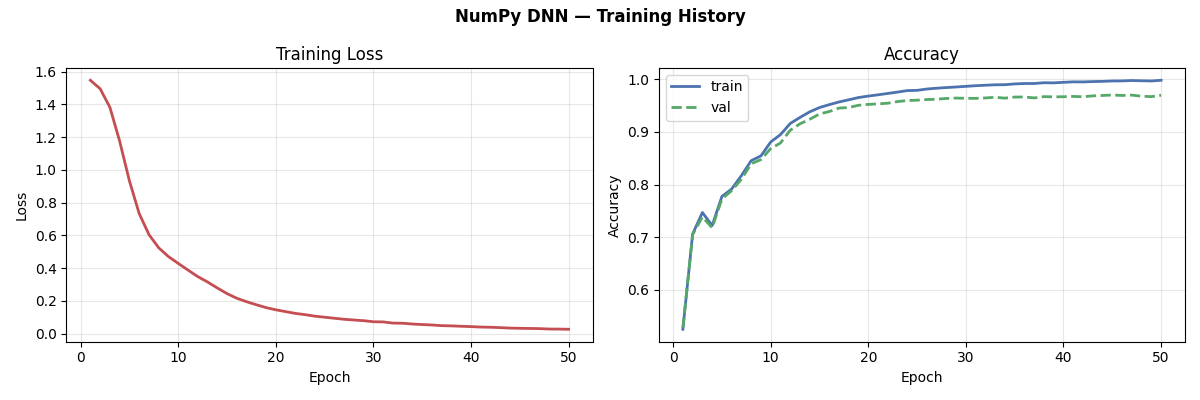
\includegraphics[width=\textwidth]{images/numpy_dnn_train.png}
\caption{Resultados do treino do modelo NumPy DNN.} \label{numpy_dnn_train}
\end{figure}

\subsection{PyTorch DNN}

O modelo PyTorch DNN foi treinado com \textit{Cross-Entropy Loss} e otimizador Adam, usando \(\text{learning\_rate}=10^{-3}\), \(\text{batch\_size}=32\) e até 10 épocas. Foi aplicado \textit{early stopping} com paciência 3, com monitorização de \textit{accuracy} de validação por época. Para análise complementar, foram calculadas métricas globais no conjunto de avaliação e acurácia por classe.

No fim do treino, os resultados são visualizados na Fig.~\ref{pytorch_dnn_train}.

\begin{figure}
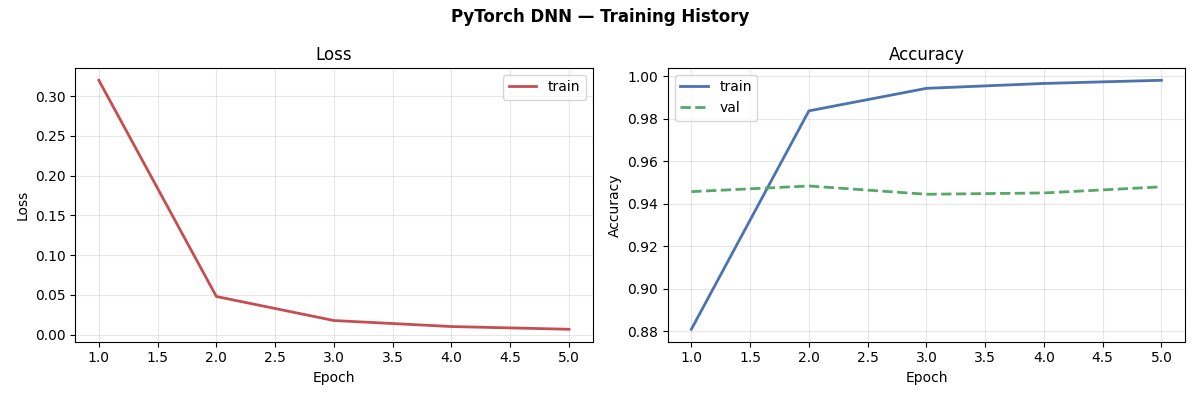
\includegraphics[width=\textwidth]{images/pytorch_dnn_train.png}
\caption{Resultados do treino do modelo PyTorch DNN.} \label{pytorch_dnn_train}
\end{figure}

\subsection{Transformer Genérico}

O Transformer genérico foi treinado com a API \textit{Trainer} da biblioteca \textit{Transformers}, com os seguintes hiperparâmetros principais: 3 épocas, \(\text{batch\_size}=32\), \(\text{learning\_rate}=2\times10^{-4}\), \textit{weight decay} de \(0.01\), \textit{warmup ratio} de \(0.1\) e \textit{scheduler} cosseno. A avaliação foi executada ao fim de cada época, com retenção automática do melhor checkpoint segundo \(F1\)-macro.

No fim do treino, os resultados são visualizados na Fig.~\ref{transformer_train}.

\begin{figure}
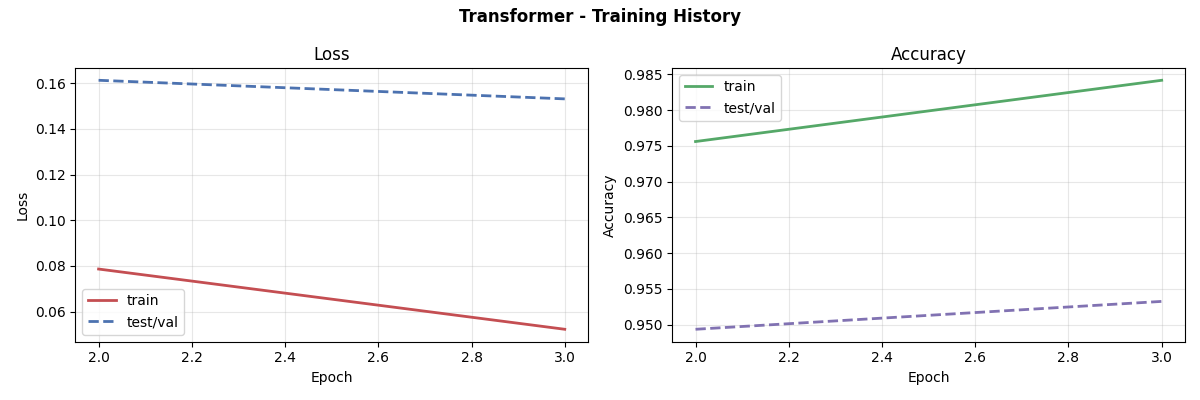
\includegraphics[width=\textwidth]{images/transformer_train.png}
\caption{Resultados do treino do modelo Transformer Genérico.} \label{transformer_train}
\end{figure}

\subsection{BERT Fine-tuning (RoBERTa-base)}

O modelo RoBERTa-base foi ajustado por \textit{fine-tuning} com \textit{Trainer}, utilizando 3 épocas, \(\text{batch\_size}=32\), \(\text{learning\_rate}=2\times10^{-5}\), \textit{weight decay} de \(0.01\), comprimento máximo de sequência 256 e acumulação de gradientes em 2 passos. A avaliação foi realizada por época, com carregamento automático do melhor modelo no final do treino segundo \(F1\)-macro.

Em termos comparativos, a avaliação final considerou consistência entre desempenho global (\textit{accuracy}/\(F1\)-macro) e estabilidade por classe, permitindo analisar o compromisso entre modelos mais leves (DNNs) e modelos baseados em \textit{Transformers}.

\section{Discussão}

Os resultados obtidos sugerem um compromisso claro entre custo computacional e capacidade de generalização. Modelos DNN baseados em vetorização TF-IDF apresentam treino mais rápido e maior simplicidade de interpretação, enquanto modelos baseados em \textit{Transformers} tendem a capturar padrões semânticos mais complexos. Em particular, a comparação entre NumPy DNN e PyTorch DNN permite isolar o impacto da infraestrutura de treino, mantendo estrutura de rede semelhante. Já a comparação entre Transformer Genérico e RoBERTa-base evidencia a vantagem potencial do \textit{transfer learning} quando há limitação de dados rotulados.

Adicionalmente, a análise por classe é essencial para interpretar desempenho real em cenário desbalanceado. Métricas agregadas podem ocultar degradações em classes minoritárias, pelo que a leitura conjunta de \textit{accuracy}, \(F1\)-macro e desempenho por classe deve orientar a seleção final do modelo.

\section{Limitações e Ameaças à Validade}

Este estudo apresenta limitações que devem ser consideradas. Primeiro, a avaliação foi baseada numa divisão estratificada única (80/20), o que pode introduzir variância associada à partição escolhida. Segundo, parte dos dados foi incorporada de forma incremental ao longo das submissões, podendo gerar diferenças de distribuição entre fases experimentais. Terceiro, apesar de terem sido comparadas arquiteturas diversas, nem todos os modelos partilham exatamente a mesma representação de entrada, o que pode afetar a comparabilidade direta.

Como ameaças à validade externa, os resultados podem não generalizar integralmente para domínios textuais distintos (e.g., textos jurídicos, biomédicos ou multilíngues). Como ameaça à validade interna, escolhas de hiperparâmetros e critério de paragem antecipada podem influenciar significativamente o desempenho reportado.

\section{Conclusão e Trabalho Futuro}

Este trabalho apresentou uma comparação sistemática entre abordagens lineares, DNNs e \textit{Transformers} para classificação de origem textual. A análise conjunta dos modelos permite concluir que arquiteturas mais simples permanecem competitivas em custo-benefício, enquanto modelos \textit{Transformer}-based oferecem maior capacidade representacional em cenários de maior complexidade semântica.

Como trabalho futuro, recomenda-se: (i) validação cruzada com múltiplas sementes para reduzir variância experimental; (ii) estudo de calibração de probabilidades e análise de incerteza; (iii) exploração de técnicas de \textit{data augmentation} textual e \textit{domain adaptation}; e (iv) inclusão de análises estatísticas de significância entre modelos para reforçar a robustez das conclusões.

%
% ---- Bibliography ----
%
% BibTeX users should specify bibliography style 'splncs04'.
% References will then be sorted and formatted in the correct style.
%
% \bibliographystyle{splncs04}
% \bibliography{mybibliography}
%
\begin{thebibliography}{12}
\bibitem{ref_article1}
Author, F.: Article title. Journal \textbf{2}(5), 99--110 (2016)

\bibitem{ref_lncs1}
Author, F., Author, S.: Title of a proceedings paper. In: Editor,
F., Editor, S. (eds.) CONFERENCE 2016, LNCS, vol. 9999, pp. 1--13.
Springer, Heidelberg (2016). \doi{10.10007/1234567890}

\bibitem{ref_book1}
Author, F., Author, S., Author, T.: Book title. 2nd edn. Publisher,
Location (1999)

\bibitem{ref_proc1}
Author, A.-B.: Contribution title. In: 9th International Proceedings
on Proceedings, pp. 1--2. Publisher, Location (2010)

\bibitem{ref_url1}
LNCS Homepage, \url{http://www.springer.com/lncs}, last accessed 2023/10/25

\bibitem{ds_openturingbench}
MLNTeam-Unical: OpenTuringBench. Hugging Face Datasets.
\url{https://huggingface.co/datasets/MLNTeam-Unical/OpenTuringBench},
último acesso em 2026/03/29.

\bibitem{ds_dahoas}
Dahoas: instruct-synthetic-prompt-responses. Hugging Face Datasets.
\url{https://huggingface.co/datasets/Dahoas/instruct-synthetic-prompt-responses},
último acesso em 2026/03/29.

\bibitem{ds_artem9k}
artem9k: ai-text-detection-pile. Hugging Face Datasets.
\url{https://huggingface.co/datasets/artem9k/ai-text-detection-pile},
último acesso em 2026/03/29.

\bibitem{ds_anthropic}
Anthropic: persuasion. Hugging Face Datasets.
\url{https://huggingface.co/datasets/Anthropic/persuasion},
último acesso em 2026/03/29.
\end{thebibliography}
\end{document}